\section{Evaluation}
\label{s:results}

%We use two distinct prototype implementations to demonstrate the
%potential performance benefits \sword\ can provide.
We use our
DPDK implementation to perform a micro-benchmark where we
explicitly manage RDMA connections to remove the atomic operations
used by Sherman's locking mechanism.  We use the P4 implementation installed on a programmable switch to show the impact of
in-flight conflict resolution at rack scale in Clover.

%We discuss the relative impact of each of our techniques across
%various workloads, and demonstrate that replacing compare-and-swap
%requests with writes eliminates hardware bottlenecks.

\subsection{Testbed} 

Our testbed consists of a rack of nine identical machines equipped
with two Intel Xeon E5-2640 CPUs and 256 GB of main memory evenly
spread across the NUMA domains. Each server is equipped with an
NVIDIA Mellanox ConnectX-5 100-Gbps NIC installed in a 16x PCIe slot and connected to a 100-Gbps ToR.  Our DPDK-based
micro-benchmarks use only three machines: a load generator, a memory
server, and a machine hosting our DPDK implementation of {\sword}.
The load generator is configured with default routing settings---it
sends traffic directly to the memory server.  We install OpenFlow
rules on a Mellanox Onyx switch to redirect the traffic to the DPDK
box.  For the P4-based Clover experiments, we replace the Onyx switch
with an Edgecore Wedge-100 programmable switch running \sword.
%Figure~\ref{fig:overview} shows the layout of our testbed.
We configure one server as a Clover memory server, one as a metadata
server, and the remaining seven as Clover clients.

\subsection{Atomic replacement}

\begin{figure}[t]
    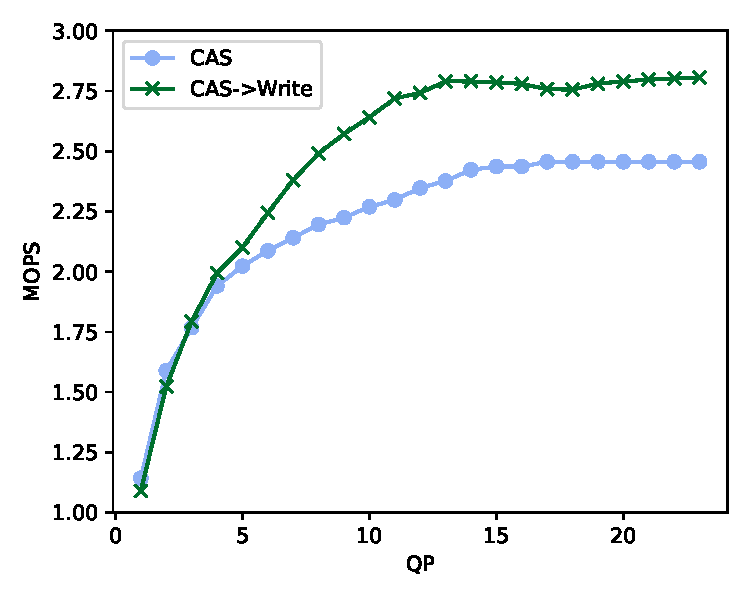
\includegraphics[width=0.485\textwidth]{fig/cas_vs_swap.pdf}
%  \vskip -0.5em
    \caption{Throughput of conflicting CAS and rewritten CAS requests as a function of client threads/QPs.}
    \label{fig:cas_vs_swap}
%      \vskip -0.5em
\end{figure}

\begin{figure*}
    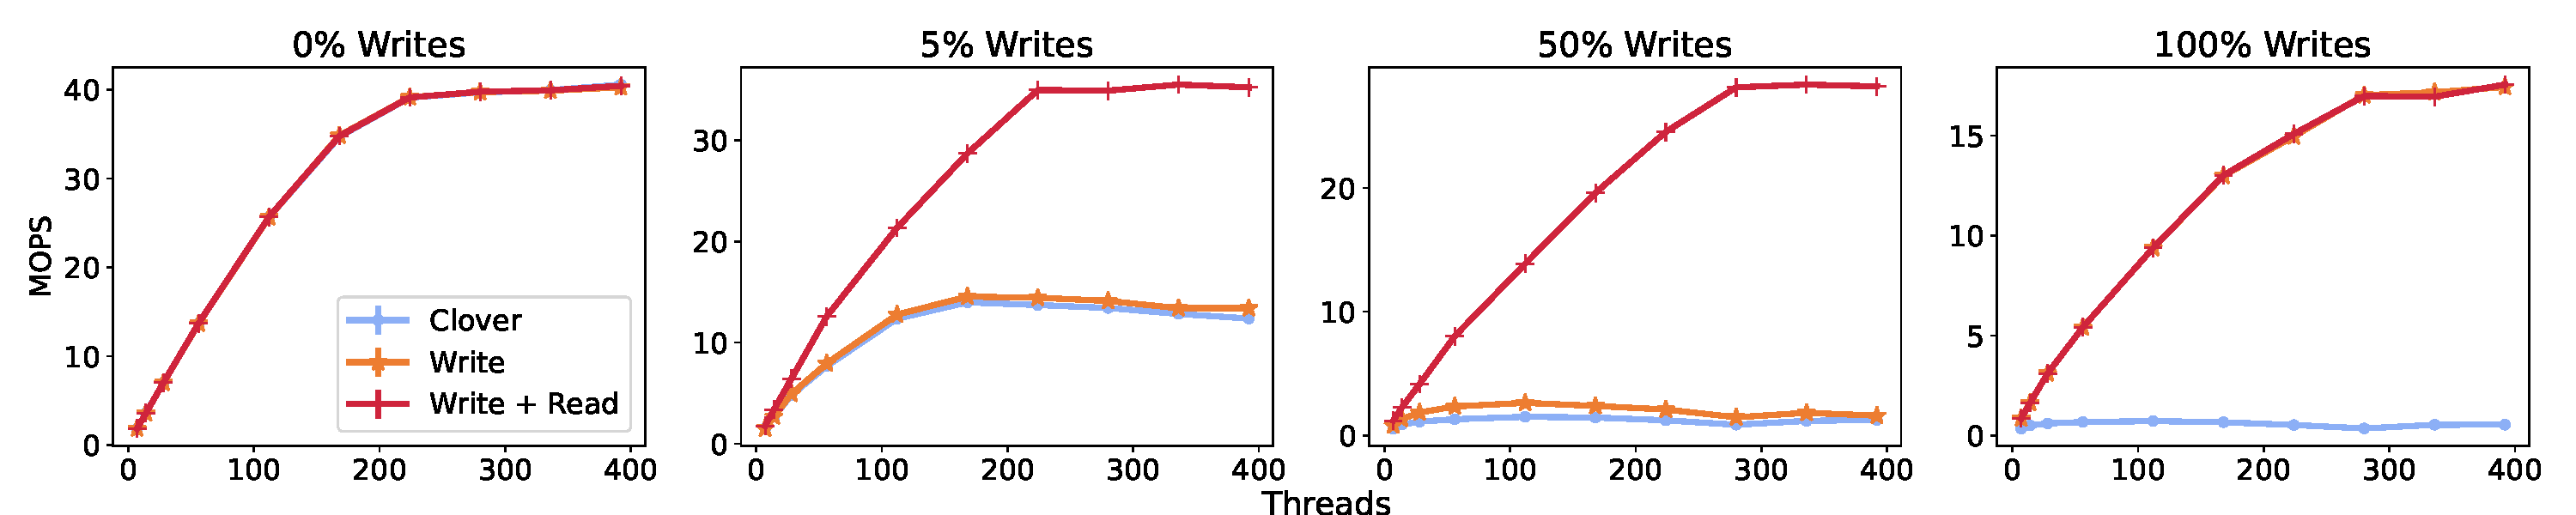
\includegraphics[width=1.0\textwidth]{fig/full_system_performance.pdf}
%  \vskip -0.5em
    \caption{Steering applied to Clover with 128-byte objects across 4 YCSB
    benchmarks. The percentage of workload writes increases from left to
    right. \sword\ throughput relative to Clover is 1.0, 2.8, 32, and 46$\times$ respectively.}
    \label{fig:full_system_performance}
      \vskip -0.5em
\end{figure*}

We show that \sword\ is able to overcome the NIC hardware bottleneck
by replacing CAS operations with writes serialized on a given QP by
running a micro-benchmark that focuses exclusively on CAS
performance. Specifically, we extract the CAS request from Sherman's
lock operation and repeatedly generate it from one client to a single
memory server (while routing it through {\sword} using OpenFlow rules).
%Here we remove clover from the
%mix and run a simple benchmark of RDMA CAS operations between two
%servers. \sword is routed to via a different set of OpenFlow rules.
Each client thread is bound to its own queue pair, and all client
threads issue CAS requests to the same shared virtual address.  We set the number of cores on the
{\sword} middlebox to 24 so that in our maximal test case each client
thread flows through exactly one middlebox core for the lowest degree
of interference between QP.

%All requests are routed
%through our middlebox.
Figure~\ref{fig:cas_vs_swap} shows the results when all requests are
directed at the same address in the remote server's main memory.  In
the default case (labeled CAS in blue), {\sword} lets CAS requests
flow through without modification, each on their own queue pair.  In
the CAS$\rightarrow$Write (green) configuration {\sword} maps all
client requests to the same QP at the server to ensure serialization
and replaces the CAS operation with a simple write.
%
%all client cores request the same address, and as such all are routed
%onto the same destination QP. Note that this configuration has the
%highest degree of contention for our middlebox as 24 client threads
%must be multiplexed to and from a single client connection. Further
%
%We measure the server throughput in terms of RDMA requests per second as we
%increase contention by adding client threads.
We see a significant increase in performance when \sword\ converts
CAS-guarded requests to QP-serialized writes.  Each configuration hits
a distinct hardware limit: CAS requests bottleneck at the server NIC
due to being applied to a single key
(c.f. Figure~\ref{fig:rdma_concur}).  When converting CAS to
serialized write operations, the bottleneck moves to the DPDK
middlebox.
%cores in our
%DPDK-based {\sword} prototype.
Specifically, DPDK requires all TX for a destination QP to be done by
the same core; hence,
%a specific core on the middlebox. Because of this
%requirement
all requests must flow through a single core prior to being forwarded, limiting the forwarding performance of our
DPDK implementation to the maximum per-core
throughput of our middlebox: 2.8 MOPS.
%In this configuration all requests to the memory server must be processed by
%the same TX core. As such our bottleneck is approximately 2.8 MOPS. Hardware
%implemented CRC, cache tuning, and better lock management for TX queues could
%yield higher per core performance in the future.
%% Despite this restriction, these results show that replacing CAS with write
%% avoids the memory server NIC's hardware bottleneck, enabling increased
%% scalability with a more performant {\sword}---such as one implemented on a
%% programmable switch. ~\sg{Our limitations here are due to programmability issues
%% on the programmable switch, multiplexing across connections inflates state
%% requirements and makes storing dynamic connection state tricky given only a
%% static number of fixed width registers.}



\subsection{Conflict avoidance}

While atomic replacement is feasible, it requires \sword\ to
explicitly manage and remap all the RDMA connections to a given (set
of) server(s)---a resource-intensive task.  Here, we consider the more
general and lightweight case where \sword\ serves as a
performance-enhancing proxy and attempts to avoid failed operations by
steering requests in flight.  We use workloads from the YCSB
benchmark~\cite{ycsb} to access 1,024 128-byte objects stored in Clover.
%a
%breakdown of our techniques, mainly read and write caching, QP mapping, and
%atomic replacement with respect to their effect to system
%% performance of four different
%% YCSB workloads. We choose YCSB-B (95\% read and 5\% write) as our baseline, and
%% YCSB-A (50\% read and 50\% write) to demonstrate how our algorithm performs
%% under high contention.  We also show the performance boosts obtained while
%% running a 100\% write workload which is intended to emulate other programmatic
%% workloads which are update heavy.

\subsubsection{Throughput}

Figure~\ref{fig:full_system_performance} shows the impact of \sword's
techniques at various levels of contention.  A read-only workload
exhibits no contention, so \sword\ simply passes through all
operations unmodified achieving a maximum throughput of approximately
40 million operations per second in our testbed.  Clover (shown in
blue) performance decreases markedly with even 5\% writes; write
steering alone (orange) provides minimal performance improvement as
the vast majority of writes succeed on their first try---it is the
reads that are failing.  Steering both reads and writes (red) restores
performance, although to a slightly lower overall throughput as even
successful Clover writes require two RDMA operations instead of one.
%Individual writes, however, can
%lead to many stale reads immediately thereafter which leads write steering
%to offer a 1.17$\times$ throughput improvement.
%
%Applying QP mapping to the
%read majorly case adds too much computational overhead to give a
%benefit when writes are low, and only a few compare and swap
%operations exist.
%
At 50\% writes, over half of all write requests fail so applying write
steering almost doubles performance.  The steered writes, however,
then out-pace reads causing the majority of reads to fail unless
\sword\ also applies read steering.  (The impact on tail latency is
clearly shown in Figure~\ref{fig:tail_latency}.)  Of course, in a
100\% write workload write steering alone is sufficient
%
%This workload leads to enough common case failures that
%performance overhead of performing QP mapping still yields a
%performance boost.
%
%in the workload.



%%\todo{real takeaways}

% \subsection{Memory Utilization}
% Our techniques give a performance boost at the cost of in network memory. We
% took special care to design our algorithms so that they could 1) use only a
% small amount of network memory, 2) be scalable depending on the resources
% available. We show how our performance varies as a function of the available in
% network state.

% As seen in Figure~\ref{fig:cache} our write caching is able to provide a
% significant performance boost while only using a small number of cached
% addresses. In the following experiment we show the maximum performance boost we
% can provide as a function of the available in network memory. Specifically in
% the case of read and write caching this means shrinking the size of the
% available cache. In terms of QP mapping it restricts the number of connections
% which can have their connections mapped. Unmapped connections must use atomic
% operations for their requests to succeed.

% \begin{figure}
%     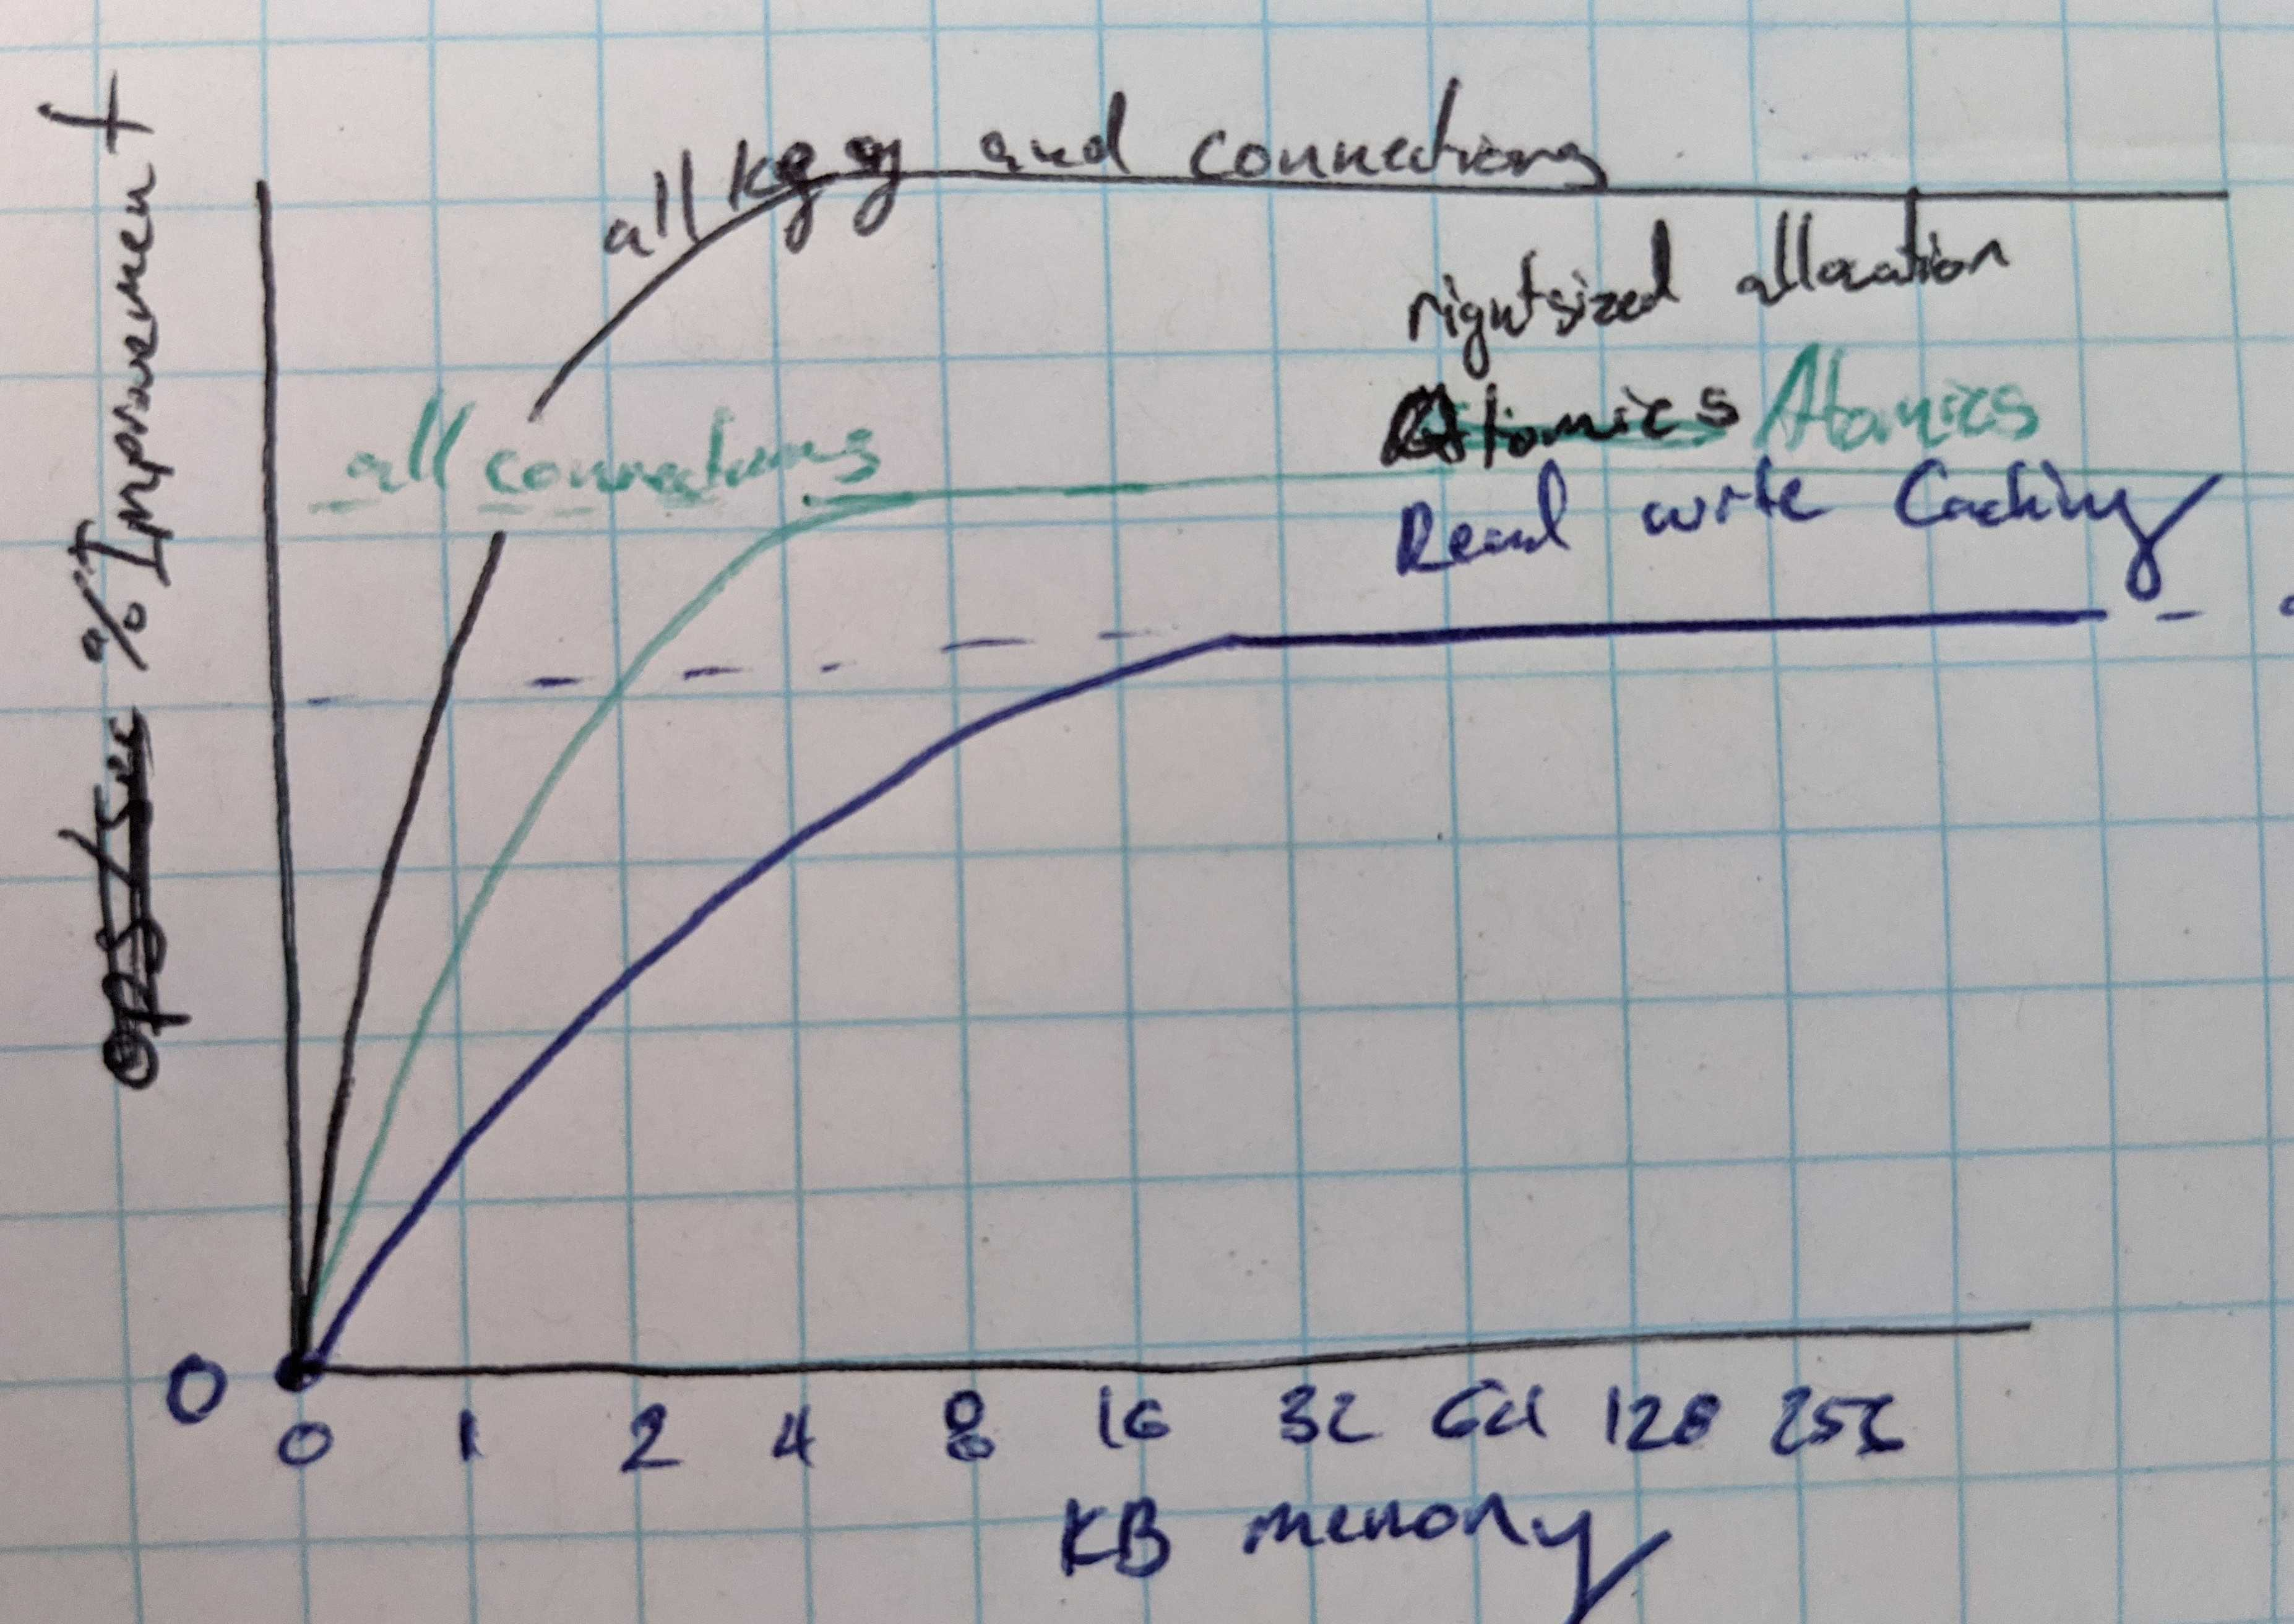
\includegraphics[width=0.45\textwidth]{fig/memory_util.jpg}
%     \caption{{Relative performance improvement of our techniques with restricted amounts of memory. Here a rightsized allocation implies that for the given number of connections we could support, all requests were mapped and reads and writes were cached.}}
%     \label{fig:memory_util}
% \end{figure}
%%\todo{say something real about the the memory utilization takeaways}


\subsubsection{Bandwidth reduction}

\begin{figure}
  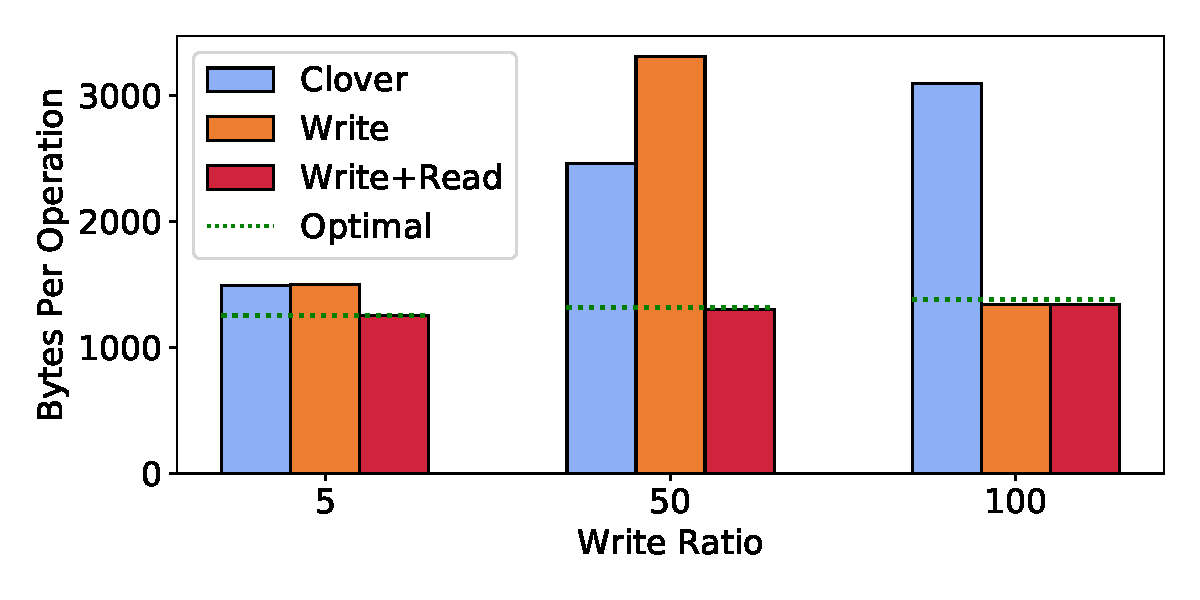
\includegraphics[width=0.485\textwidth]{fig/bandwidth_reduction.pdf}
  \centering
   \vskip -0.5em
    \caption{Average number of bytes required per Clover
      operation on 128-byte objects using each of the three techniques at various write
      intensities.}
    \label{fig:bandwidth_reduction}
     \vskip -0.5em
\end{figure}




%Placing memory operations in-band with regular network traffic can be
%problematic as applications' remote memory usage has the potential to
%vary dramatically per application.
Under contention, Clover's remote operations can require additional
packet exchanges which inflate the bandwidth necessary to service the
same number of memory accesses.  \sword's steering algorithms
remove the need for requests to retry, eliminating the overhead.
%
%Figure~\ref{fig:bandwidth_reduction} shows the average bytes
%per Clover operation under three different workloads for default
%Clover as well as {\sword}'s two steering techniques.
%
%% We calculate the optimal expected cost of a Clover operation by
%% averaging the cost of a successful operation across reads and
%% writes. We get the weighted average by multiplying the cost of a read
%% and write by the appropriate workload percentage. Each write consists
%% of an RDMA write followed by a CAS, along with the responses for each
%% message. A read consists of an RDMA read and read response, and
%% usually an additional metadata read made asynchronously with the main
%% read to fetch the latest position of the tail in case the first memory
%% read fails. Clover performs this second read opportunistically (in
%% around 99 percent of all reads in these workloads), however sometimes
%% it is omitted leading to a small over-approximation in our estimate of
%% ``optimal''.
%
Figure~\ref{fig:bandwidth_reduction} plots the average bytes per
operation for each strategy across the three workloads with writes.
(The read-only workload, not shown, never needs to retry.) We calculate the value
for each technique by summing the total bandwidth across a run and
dividing by the number of operations. Clover's bandwidth usage
increases with contention, growing by 2.5$\times$ at 5\% and
16$\times$ at 50\% writes---all of which is recovered by applying
read and write steering. Write steering alone causes significant
inflation in the cost of operations at 50\% writes because many read
requests fail as discussed above.

\subsubsection{Tail latency}

\begin{figure}
    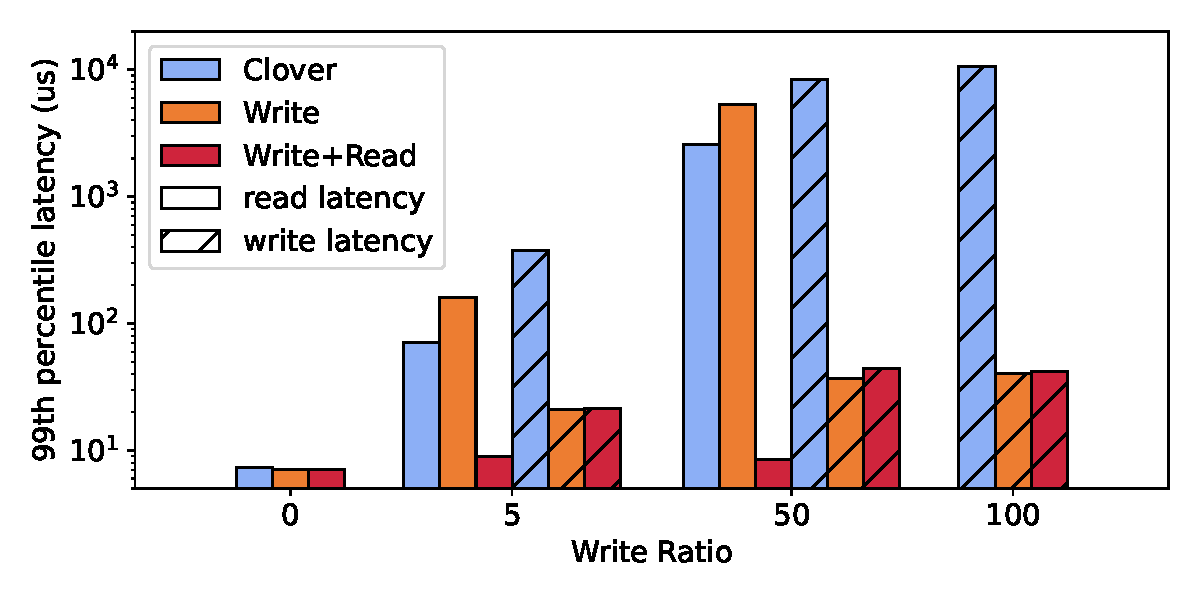
\includegraphics[width=0.485\textwidth]{fig/99th_latency_dense.pdf}
%\vskip -1em
    \caption{99th-percentile tail latencies of read (solid) and write
      (striped) Clover operations at various write intensities. (Note logarithmic $y$ axis.)}
    \label{fig:tail_latency}
      \vskip -0.5em
\end{figure}

%% Perhaps the most critical variable that governs overall system % performance
%is tail latency. In the context of disaggregated memory % systems, reads and
%writes are often deeply integrated into the % computational logic of a program
%and the whole program must wait for a % page fault to complete before
%continuing. We therefore consider poor % tail latency to be a fundamental
%barrier to the widespread adoption of % far memory systems.
Optimistic concurrency is well known to exhibit poor tail latency under
contention, and Clover is no exception.  \sword\ significantly reduces latency
as steering ensures that nearly all requests succeed on the first try.
%
Figure~\ref{fig:tail_latency} shows the 99th-percentile tail latencies
associated with \sword's read and write steering in comparison to default Clover
at varying write intensities. Clover's p99 read latency (solid blue) at 5\%
writes is 70~$\mu$s, around 10$\times$ its baseline our our testbed. With read
and write steering (solid red) the read tail latency drops to 8~$\mu$s---a
8$\times$ improvement over Clover even in this low-contention regime. At 50\%
writes the performance increase from steering increases dramatically: p99 read latency drops by over 300$\times$.
%% As discussed above, in either % case applying write steering alone actually
%hurts performance, as it % makes reads more likely to fail.  % %read
%performance is improves by 2$\times$ % %relative to Clover with the exception
%of write steering alone. When % %write steering is applied without the aid of
%read steering the writes % %quickly out-pace the reads, leading the vast
%majority of reads to fail % %on their first attempt.  % Given that these tests
%were conducted with a % Zipf distribution across 64 cores it is highly likely
%that more than % one thread is writing to the hottest keys at any point during
%the % run. This leads some read requests to fail 10s of times before %
%succeeding.
%
%Because of this property we suggest that read and write steering be used in
%concert unless the workload is explicitly known.
%
Writes (hashed) have slightly more than double the latency of reads as they
require two round trips and atomics are slower to execute than other operations.
Combined write and read steering provides a 17, 189, and 252$\times$ improvement
in write tail latency, respectively, across 5, 50, and 100\% write workloads.
As one might expect, performing write steering alone privileges writes over
reads, dropping their tail latencies slightly further---at the cost of a
dramatic spike in read tail latency.

%% Figure~\ref{fig:tail_latency} also shows the performance of queue pair
%% mapping and atomic replacement (CAS$\rightarrow$Write) when applied in addition
%% to write+read steering.  Because the requests are already likely to
%% succeed, there is no reason to expect any significant drop in tail
%% latency by vectoring the requests to a particular QP or removing the
%% CAS guard.  Rather, these plots show that the (significant) 
%% logic required in {\sword} to implement these functions result in only
%% marginal increase in tail latency relative to steering alone---and still
%% significantly outperforms Clover alone.


%The application of QP mapping and swapping
%CNS to writes does little to effect tail latency as their performance
%cost comes largely as an increase to the average.

\subsubsection{Partial steering}

\begin{figure}
    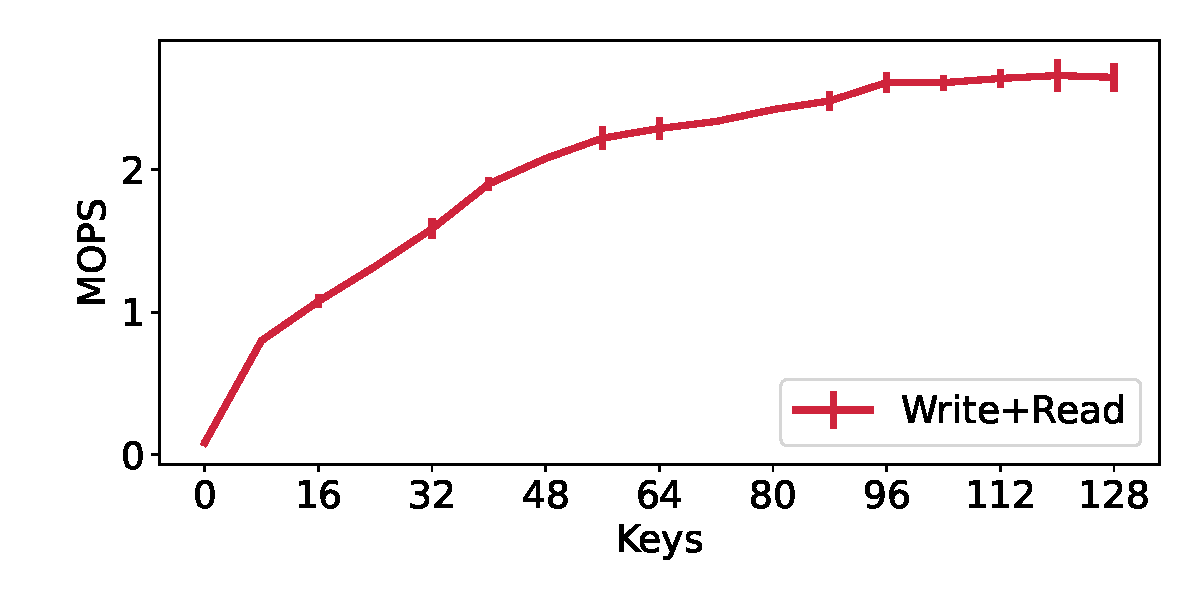
\includegraphics[width=0.485\textwidth]{fig/keys_tracked.pdf}
%\vskip -1em

    \caption{Per-client throughput as a function of the number of
      Clover keys \sword\ steers.  50:50 workload averaged 
      across 6 hosts each running 56 threads.  }

    \label{fig:keys_tracked}
      \vskip -0.5em
\end{figure}

One of most appealing aspects of \sword's steering is the fact that it
need not be applied to all servers, or even memory regions (i.e.,
Clover keys) of a given server.
%In the presence of heavy-tail
%workloads, even steering accesses to a msall number of hot (i.e.,
%highly contended) keys can provide a major performacne boost.
Figure~\ref{fig:keys_tracked} shows per-client throughput as a
function of the number of keys steered by \sword.  To accentuate the
impact, we use a Zipf parameter of 1.5---as opposed to 0.99 in prior
experiments---to enhance the locality of requests.  (See Appendix~\ref{ss:zipf} for a full range.)
%If a programs state is too large to cache on a switch (millions of keys) but a
%few hot keys are highly contested, {\sword} can still provide significant
%benefits by acting on only on the contested state. In the following experiment
%we track a subset of Clovers keys, allowing the rest to flow through
%uninterrupted. In this experiment we run clover at a zipf of 1.5 (most requests
%are on lower keys). We add keys to \sword's tracking list in order of hotness by
Steering requests for only the hottest-8 keys provides a 9.5$\times$
improvement while tracking the hottest 64 delivers
27$\times$.
%; maximum performance boost (i.e., tracking all keys, not shown) is
%(c.f. Figure~\ref{fig:contention}).



